\section{Experiments}
\label{sec:exp}

\subsection{Controlled tasks}

We first relate task structure to the gap between a fusing model and a linear readout in a controlled setting. We
build $10\times10$ answer tables over pairs of CIFAR-100 classes and select 63 tables with PID synergy between 0.40 and
0.75 bits, chosen so that synergy and structure are nearly uncorrelated. For each table we train a full model and a
linear readout on frozen features (three seeds). The readout gap follows the exception share: the partial rank
correlation with exception share, controlling for synergy, is $+0.91$ $[0.83,0.94]$, against $+0.22$ $[-0.06,0.45]$ for
synergy controlling for exception share. Tables with no exceptions carry up to 0.67 bits of synergy, yet their gap never
exceeds 9 points. A replication on 62 new tables gives the same pattern ($+0.86$ versus $+0.11$). The same holds with
$I_{\mathrm{ccs}}$ and MMI (Sec.~\ref{sup:controlled}). Note that the readout gap is itself bounded by the ceiling
(Prop.~\ref{prop:ceiling}), so this experiment shows that trained readouts approach the bound, not that structure
predicts behaviour beyond it; the next experiment separates the two.

\subsection{Modern VLMs}
\label{sec:vlm}

\paragraph{Setup.}
We build 99 complete answer tables of 10 questions and 100 images, with every question well posed on every image: 24
CLEVR, 24 GQA, 43 CLOVE and 8 POPE tables. On GQA, CLOVE and POPE only existence questions qualify, so their exceptions
mostly encode which objects co-occur in which images (Sec.~\ref{sup:tables}). The rule is proven optimal for 95 tables.
We evaluate four 7--8B VLMs from different families: Qwen2.5-VL-7B~\cite{bai2025qwen25vl},
InternVL3.5-8B~\cite{wang2025internvl35}, LLaVA-OneVision-1.5-8B~\cite{an2025llavaov15} and
Idefics3-8B~\cite{laurencon2024building}, zero-shot on every cell, scoring each cell by the log-odds of ``yes'' versus
``no'', and compute the EMAP drop per table.

\paragraph{All four VLMs use interactions.}
All four models lose accuracy when their interactions are removed (Tab.~\ref{tab:vlm_acc}), most on CLEVR, whose tables
are the least additive. Prop.~\ref{prop:floor} holds on every model and table, as it must; it is a sanity check of the
pipeline, and it is vacuous where a model's error exceeds the exception share (\eg Idefics3 on CLEVR, error $0.13$
against $s\approx0.10$).

\begin{table}[t]
\centering\small\setlength{\tabcolsep}{4pt}
\caption{Zero-shot accuracy / EMAP drop on the confirmatory sub-tables. In brackets: mean additive ceiling $C(T)$.}
\label{tab:vlm_acc}
\begin{tabular}{lcccc}
\toprule
Model & CLEVR & GQA & CLOVE & POPE \\
      & (0.90) & (0.93) & (0.94) & (0.98) \\
\midrule
Qwen2.5-VL-7B   & 0.90 / .16 & 0.94 / .06 & 0.93 / .06 & 0.98 / .03 \\
InternVL3.5-8B  & 0.98 / .20 & 0.90 / .06 & 0.86 / .05 & 0.93 / .00 \\
LLaVA-OV-1.5-8B & 0.99 / .17 & 0.95 / .06 & 0.93 / .06 & 0.97 / .02 \\
Idefics3-8B     & 0.87 / .12 & 0.93 / .05 & 0.91 / .05 & 0.97 / .02 \\
\bottomrule
\end{tabular}
\end{table}

\paragraph{Separating structure from synergy.}
On the original tables, exception share predicts the EMAP drop within CLEVR ($\rho$ up to $+0.97$) and CLOVE ($+0.58$
to $+0.76$) but not GQA ($\approx0.1$ for all models), and synergy does almost as well, because the two measures are
strongly correlated on natural tables ($+0.88$ to $+0.95$ within benchmark). We therefore select, from 27 candidate
50-image subsets per table and using the answer tables only, one sub-table per table such that within each benchmark
the exception share is uncorrelated with synergy (study B) or with both synergy and the yes-share (study C). In study B,
both measures kept a signal; synergy's followed the yes-share ($+0.57$ to $+0.83$). Study C was pre-registered with a
model we had not examined (Idefics3). With synergy, accuracy and yes-share held fixed, exception share ranks tables by
EMAP drop (partial $\rho=+0.42$ $[0.21,0.56]$) and synergy adds no signal ($+0.07$ $[-0.17,0.29]$). InternVL3.5 shows
the same pattern; for LLaVA-OV-1.5 synergy keeps a signal ($+0.24$ $[0.02,0.42]$) and for Qwen2.5-VL the structural
effect is weaker ($+0.26$). Answer balance itself carries a signal for every model (partial $\rho$ of the yes-share
$+0.23$ to $+0.34$, all intervals above zero). Partialling out the yes-share removes variance that synergy shares with
it, so the comparison is between structure and the part of synergy not explained by answer balance. In a linear
regression, neither measure explains more than 1--4\% of variance beyond benchmark and answer balance: the effect is a
ranking within benchmarks.

\paragraph{How much of this does accuracy alone require?}
Prop.~\ref{prop:floor} ties the EMAP drop of an accurate model to $s$, so part of any correlation is arithmetic. We
measure it with a null scorer that has each model's accuracy on yes and no cells of each table but no structure in its
errors: logits $(2T_{ab}-1)\mu_y+\varepsilon_{ab}$, $\varepsilon\sim\mathcal N(0,1)$, with $\mu_y$ set to match the
model's per-answer accuracy, run through the identical pipeline (20 draws). Tab.~\ref{tab:null} shows that the null
reproduces most of the relation (pre-registered test on Idefics3: fail). Interaction dependence beyond what accuracy
requires tracks structure only for InternVL3.5, whose mean EMAP drop is also twice the null's ($.086$ vs $.044$); for
the other three models it is close to the null ($\le .009$ apart). The defensible reading is therefore that the
exception share predicts the interaction dependence an accurate solution \emph{requires}, and that current VLMs mostly
depend on interactions about as much as their accuracy demands.

\begin{table}[t]
\centering\small\setlength{\tabcolsep}{3pt}
\caption{Study C sub-tables. Within-benchmark partial rank correlation with $s$ (controls: synergy, accuracy,
yes-share), for the observed EMAP drop $\Delta$, for an accuracy-matched null scorer $\Delta_0$, for the excess
$\Delta-\Delta_0$, and for the slack $\Delta-(s-e)$; 95\% bootstrap intervals over tables.}
\label{tab:null}
\begin{tabular}{lcccc}
\toprule
Model & $\Delta$ & $\Delta_0$ (null) & $\Delta-\Delta_0$ & slack \\
\midrule
Idefics3     & $+.42$ & $+.37$ & $+.17$ $[-.07,.38]$ & $-.14$ \\
InternVL3.5  & $+.42$ & $+.50$ & $+.26$ $[.05,.43]$  & $+.28$ $[.06,.45]$ \\
LLaVA-OV-1.5 & $+.43$ & $+.40$ & $+.12$ $[-.11,.32]$ & $-.05$ \\
Qwen2.5-VL   & $+.26$ & $+.30$ & $+.05$ $[-.17,.25]$ & $-.09$ \\
\bottomrule
\end{tabular}
\end{table}

\paragraph{Which cells require interactions?}
At the cell level we predict which answers change when interactions are removed. The graded misfit does so with AUC
$0.78$--$0.88$, above the model's own confidence ($0.63$--$0.73$). The binary exception label does not (AUC $0.60$--$0.66$
with stable labels, $0.64$--$0.71$ counting any optimal rule's exceptions), because exceptions are a small and
non-unique set while flips also occur next to them (Sec.~\ref{sup:unique}).

\section{What Continual Learners Lose}
\label{sec:cl}

\paragraph{Setup.}
Each model learns one task and then another, and we measure how much of the first task is retained and how well the
second is learned. Tasks are constructed answer tables, pairs of CLEVR question families (40 runs), pairs of GQA
existence families (24 units, three seeds) and the six CLOVE scene tasks~\cite{lei2023symbolic} (six orders, two seeds).
Each model fuses frozen image and question features through two small trainable encoders and a fusion head. This is far
from a VLM; Sec.~\ref{sec:cl} ends with a VLM study. We compare twelve methods: finetuning; EWC~\cite{kirkpatrick2017overcoming},
SI~\cite{zenke2017continual}, LwF~\cite{li2017learning} and feature distillation; ER~\cite{chaudhry2019tiny},
A-GEM~\cite{chaudhry2019efficient}, GEM~\cite{lopezpaz2017gradient}, DER++~\cite{buzzega2020dark} and
iCaRL~\cite{rebuffi2017icarl} with a buffer of 1{,}000 samples; and DER-expansion~\cite{yan2021der} and multiple heads.
Regularisation strengths keep learning of the second task within 2 points of finetuning.

\begin{table*}[t]\centering\scriptsize\setlength{\tabcolsep}{2.2pt}
\caption{\textbf{Standard vs.\ exception-aware continual-learning metrics.} ACC, BWT and exception accuracy (E-ACC) in
points; best, second and third per column in \textcolor{red!75!black}{red}, \textcolor{blue!70!black}{blue},
\textcolor{green!45!black}{green}. $\Delta$B and $\Delta$F: same-answer gap (exceptions minus rule cells) in backward /
forward transfer; \textbf{bold}: 95\% interval below zero. E-ACC below 50 is expected for a model that has learned the
additive rule, which is wrong on exceptions by definition. $\Delta$F on constructed tasks is omitted (--): the second
table's exception cells are not unique (Sec.~\ref{sup:unique}). Difficulty-matched gaps are in Tab.~\ref{tab:difficulty}.}
\label{tab:main}\resizebox{\textwidth}{!}{\begin{tabular}{ll|rrrrr|rrrrr|rrrrr|rrrrr}\toprule
\textbf{Method} & \textbf{Extra signal} & \multicolumn{5}{c}{\textbf{Constructed}} & \multicolumn{5}{c}{\textbf{CLEVR}} & \multicolumn{5}{c}{\textbf{GQA}} & \multicolumn{5}{c}{\textbf{CLOVE-scene}}\\
 & & ACC$\uparrow$ & BWT$\uparrow$ & E-ACC$\uparrow$ & $\Delta$B$\uparrow$ & $\Delta$F$\uparrow$ & ACC$\uparrow$ & BWT$\uparrow$ & E-ACC$\uparrow$ & $\Delta$B$\uparrow$ & $\Delta$F$\uparrow$ & ACC$\uparrow$ & BWT$\uparrow$ & E-ACC$\uparrow$ & $\Delta$B$\uparrow$ & $\Delta$F$\uparrow$ & ACC$\uparrow$ & BWT$\uparrow$ & E-ACC$\uparrow$ & $\Delta$B$\uparrow$ & $\Delta$F$\uparrow$\\\midrule
\rowcolor{gray!12}\multicolumn{22}{l}{\textbf{Reference}}\\
Finetune & None & 66.0 & -39.1 & 66.4 & 11.2 & -- & 73.2 & -29.6 & \textcolor{blue!70!black}{\textbf{51.5}} & 33.5 & 1.4 & 88.8 & -5.3 & 46.2 & 2.0 & -2.8 & 83.5 & -7.5 & 31.0 & 16.8 & -0.1\\
\rowcolor{gray!12}\multicolumn{22}{l}{\textbf{Regularisation (parameter)}}\\
EWC & Fisher & 66.7 & -37.1 & 66.8 & 10.8 & -- & 74.2 & -27.7 & 50.2 & 31.8 & 0.6 & 89.5 & -3.9 & 47.2 & 1.1 & -3.1 & 85.8 & -4.5 & 24.9 & 18.5 & \textbf{-1.7}\\
SI & Path integral & 67.1 & -36.0 & 68.3 & 13.6 & -- & 75.8 & -24.0 & 48.0 & 24.9 & \textbf{-4.9} & 89.6 & -3.4 & 45.3 & -1.6 & \textbf{-5.7} & 87.1 & -2.8 & 27.1 & 14.4 & -2.8\\
\rowcolor{gray!12}\multicolumn{22}{l}{\textbf{Regularisation (distillation)}}\\
LwF & Logit distill. & \textcolor{green!45!black}{\textbf{75.8}} & -13.3 & \textcolor{green!45!black}{\textbf{70.8}} & 0.4 & -- & 75.6 & -20.1 & 46.4 & 22.2 & 1.8 & 89.8 & -2.9 & 36.6 & 9.9 & \textbf{-7.1} & 86.7 & -3.7 & 22.9 & 18.6 & 1.3\\
Feature distill. & Feature distill. & 64.1 & -39.0 & 64.7 & 12.4 & -- & 72.7 & -26.8 & 43.3 & 32.3 & \textbf{-13.2} & 88.7 & -5.4 & 37.6 & 4.5 & \textbf{-7.5} & 84.9 & -4.7 & 20.8 & 24.7 & \textbf{-6.8}\\
\rowcolor{gray!12}\multicolumn{22}{l}{\textbf{Memory / replay}}\\
ER & Buffer & \textcolor{blue!70!black}{\textbf{78.2}} & -13.6 & \textcolor{blue!70!black}{\textbf{72.5}} & -1.3 & -- & \textcolor{blue!70!black}{\textbf{85.7}} & \textcolor{green!45!black}{\textbf{-2.1}} & 45.5 & \textbf{-8.7} & \textbf{-6.0} & \textcolor{blue!70!black}{\textbf{90.9}} & \textcolor{green!45!black}{\textbf{-0.5}} & \textcolor{red!75!black}{\textbf{54.7}} & 1.1 & -1.3 & 86.8 & -3.6 & 33.8 & 3.8 & 0.5\\
A-GEM & Buffer + grad. proj. & 73.6 & -23.5 & 70.3 & 3.0 & -- & 84.8 & -6.0 & 46.5 & \textbf{-11.0} & -0.7 & 90.6 & -1.5 & 52.9 & -0.7 & -2.6 & \textcolor{green!45!black}{\textbf{87.5}} & \textcolor{green!45!black}{\textbf{-2.6}} & 33.9 & 4.2 & 0.1\\
GEM & Buffer + grad. QP & 74.5 & -21.4 & 70.4 & 2.4 & -- & 84.7 & -6.3 & 46.7 & \textbf{-10.0} & -0.4 & \textcolor{green!45!black}{\textbf{90.8}} & -1.0 & 53.3 & -1.6 & -2.9 & 85.6 & -4.8 & \textcolor{blue!70!black}{\textbf{36.4}} & 7.4 & 0.1\\
DER++ & Buffer + logits & 75.1 & \textcolor{red!75!black}{\textbf{-2.1}} & 68.8 & \textbf{-1.1} & -- & \textcolor{green!45!black}{\textbf{85.5}} & \textcolor{red!75!black}{\textbf{0.1}} & 34.9 & \textbf{-9.2} & \textbf{-25.6} & 90.5 & \textcolor{red!75!black}{\textbf{0.3}} & 49.7 & \textbf{-2.6} & \textbf{-7.1} & \textcolor{red!75!black}{\textbf{89.4}} & \textcolor{red!75!black}{\textbf{-0.7}} & 26.7 & 0.3 & -1.5\\
iCaRL & Herding + NME & 71.9 & \textcolor{green!45!black}{\textbf{-10.6}} & 53.7 & \textbf{-28.7} & -- & 72.5 & -15.8 & 39.0 & \textbf{-7.8} & -6.6 & 80.0 & -12.2 & \textcolor{blue!70!black}{\textbf{54.7}} & \textbf{-16.7} & \textbf{-15.7} & 78.0 & -5.4 & \textcolor{red!75!black}{\textbf{47.4}} & 7.6 & -1.4\\
\rowcolor{gray!12}\multicolumn{22}{l}{\textbf{Architectural}}\\
DER (expansion) & Frozen encoders + buffer & \textcolor{red!75!black}{\textbf{80.5}} & \textcolor{blue!70!black}{\textbf{-9.3}} & \textcolor{red!75!black}{\textbf{76.5}} & 1.9 & -- & \textcolor{red!75!black}{\textbf{87.6}} & \textcolor{blue!70!black}{\textbf{-0.3}} & \textcolor{red!75!black}{\textbf{51.5}} & -1.6 & \textbf{-4.8} & \textcolor{red!75!black}{\textbf{91.6}} & \textcolor{blue!70!black}{\textbf{0.3}} & \textcolor{green!45!black}{\textbf{54.3}} & -0.9 & -2.7 & \textcolor{blue!70!black}{\textbf{87.7}} & \textcolor{blue!70!black}{\textbf{-2.1}} & \textcolor{green!45!black}{\textbf{34.7}} & 1.2 & -0.0\\
Multi-head & Task ID & 73.9 & -23.6 & 66.5 & \textbf{-4.7} & -- & 82.5 & -12.2 & \textcolor{green!45!black}{\textbf{50.4}} & 0.1 & 5.1 & 88.6 & -6.0 & 47.9 & \textbf{-7.6} & -2.4 & 83.6 & -7.7 & 33.8 & 4.4 & 1.3\\
\bottomrule\end{tabular}}\end{table*}

\begin{figure*}[t]\centering
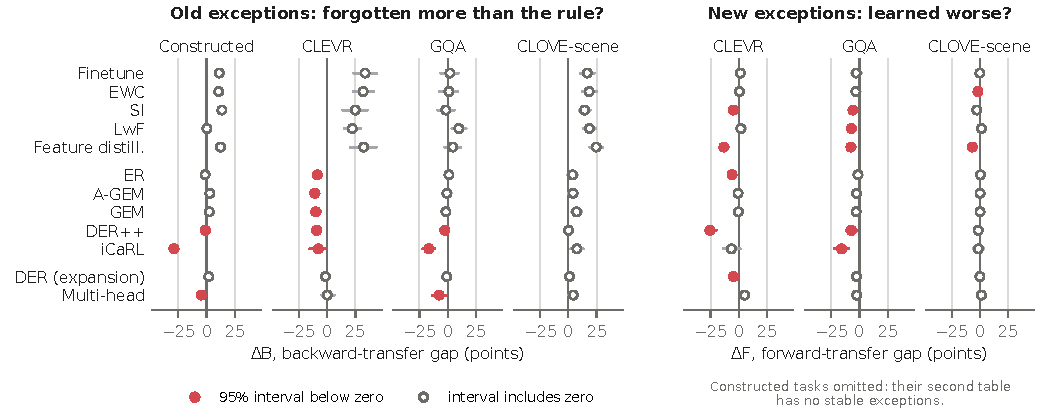
\includegraphics[width=\linewidth]{fig/fig_gaps.pdf}
\caption{\textbf{Exceptions against rule cells with the same answer, for the old task and the new one.}
Gap in backward transfer ($\Delta$B, left) and forward transfer ($\Delta$F, right) between exceptions and rule cells
with the same answer, per method and benchmark, with 95\% intervals; filled: interval below zero. \emph{Old
exceptions} are forgotten faster than the rule on CLEVR by every replay method; elsewhere the gap is small or absent
once answers are matched. Positive gaps for finetuning and weak regularisers vanish once difficulty is matched
(Tab.~\ref{tab:difficulty}). \emph{New exceptions} are learned worse than the new rule by most protective methods on
CLEVR and GQA; the constructed-task forward panel is omitted because that table's exceptions are not unique.}
\label{fig:gaps}\end{figure*}

\paragraph{Comparing exceptions and rule cells.}
Three confounds must be removed before comparing exceptions with rule cells. \emph{Answer:} in the existence tasks
92\% (GQA) and 89\% (CLOVE) of exceptions are ``yes'' against 6--8\% of rule cells, and models drift toward the
majority answer; we therefore compare within each answer and average the differences, weighting each answer by its
share among exceptions ($\Delta$B, $\Delta$F; negative means exceptions are forgotten, or learned, worse). \emph{Difficulty:}
exceptions are atypical by construction, and atypical examples are known to be learned late and forgotten
early~\cite{toneva2019empirical,feldman2020does,shah2020pitfalls}; we therefore also match on difficulty, comparing
exceptions with rule cells of the same answer in the same decile of the model's margin for the true answer (the
first-task model's margin for forgetting, a second-task-only model's margin for learning; Tab.~\ref{tab:difficulty}).
\emph{Labels:} exception sets are not unique (Sec.~\ref{sec:theory}); we repeat the key comparisons with stable labels.

\paragraph{Old exceptions are forgotten faster on compositional tasks.}
On CLEVR, replay methods forget old exceptions faster than rule cells with the same answer: by 8.7 to 11.0 points for
ER, A-GEM, GEM and DER++, all intervals below zero. The result holds with stable labels only ($-9.3$ to $-12.0$) and,
for the methods we re-ran, with difficulty matched: ER $-12.5$ $[-14.5,-10.4]$, DER++ $-7.8$ $[-9.6,-5.6]$,
DER-expansion $-4.2$ (pre-registered: pass). The positive gaps of finetuning and weak regularisers vanish once
difficulty is matched (finetuning $+21.6\to+0.2$): they lose almost everything, and exceptions, which start near chance,
have less to lose. On GQA and CLOVE the gap largely disappears after matching answers, so the raw gap there was mainly
answer imbalance.

\paragraph{Exceptions are learned worse.}
After learning one task, models learn the next task's exceptions worse than its rule cells. On CLEVR this holds for
every method once difficulty is matched, from $-10.6$ (finetuning) to $-27.0$ (DER++) points, and with stable labels
(DER++ $-27.8$). On GQA the evidence is weak: matched rule cells exist for only 18--19\% of exceptions (exceptions there are mostly ``yes'' cells the models miss, while ``yes'' rule cells are rarely missed), the re-run's unmatched DER++ gap is not significant ($-3.3$ $[-9.5,3.3]$), and its difficulty-matched gap is $-9.5$ $[-18.6,-0.0]$. Our pre-registered difficulty test, which counted constructed tasks, CLEVR and GQA, passed, but given the label ambiguity on the constructed tasks and the low coverage on GQA we regard the learning result as established on CLEVR only. On the
constructed tasks the gap cannot be interpreted: the second task's table is a balanced random table on which every cell
is an exception under some optimal rule and a rule cell under another. On CLOVE the gap is small for most methods.

\begin{table}[t]
\centering\small\setlength{\tabcolsep}{3pt}
\caption{Difficulty-matched gaps on CLEVR (points; exceptions minus rule cells with the same answer and the same
margin decile; 95\% bootstrap intervals over units; 99\% of exceptions have matched rule cells). GQA, where only
18--19\% of exceptions can be matched, is in Sec.~\ref{sup:difficulty}.}
\label{tab:difficulty}
\begin{tabular}{lcccc}
\toprule
 & \multicolumn{2}{c}{Backward (forgetting)} & \multicolumn{2}{c}{Forward (learning)} \\
Method & same answer & + difficulty & same answer & + difficulty \\
\midrule
Finetune      & $+21.6$ & $+0.2$ $[-4.8,5.0]$   & $+1.9$  & $-10.6$ $[-12.9,-8.4]$ \\
LwF           & $+16.9$ & $-1.5$ $[-5.7,2.4]$   & $+0.1$  & $-11.7$ $[-14.3,-9.5]$ \\
Feature dist. & $+17.3$ & $-0.7$ $[-6.6,4.6]$   & $-10.9$ & $-22.8$ $[-25.4,-20.2]$ \\
ER            & $-8.3$  & $-12.5$ $[-14.5,-10.4]$ & $-4.9$ & $-17.4$ $[-20.2,-14.6]$ \\
DER++         & $-6.5$  & $-7.8$ $[-9.6,-5.6]$  & $-17.2$ & $-27.0$ $[-31.6,-21.8]$ \\
DER-expansion & $-2.4$  & $-4.2$ $[-6.2,-2.3]$  & $-2.7$  & $-14.0$ $[-16.5,-11.6]$ \\
\bottomrule
\end{tabular}
\end{table}

\paragraph{Standard metrics hide the difference.}
Because exceptions are a small part of the data, backward transfer gives them little weight. On CLEVR, DER++ has the
best overall backward transfer ($+0.1$ points) yet the lowest exception accuracy among replay methods (34.9). Values
below 50 are expected for any model that has learned the rule, which is wrong on exceptions by definition; what matters
is the comparison across methods. DER-expansion, which freezes the old encoders, has the best overall accuracy on three
of four benchmarks and loses exceptions least among replay-based methods.

\paragraph{Replaying exceptions helps.}
DER++ buffers of the same size and answer balance, filled either at random or half with exception cells
(pre-registered): the exception-focused buffer keeps 6.8 to 8.5 points more old exceptions on the constructed tasks,
CLEVR and CLOVE, but not on GQA, where answer balance alone explains the gain. It costs 1--3 points of overall backward
transfer (the pre-registered cost bound failed on two benchmarks).

\begin{table}[t]
\centering\small\setlength{\tabcolsep}{4pt}
\caption{VLM continual learning on CLOVE-scene (six tasks; Qwen2.5-VL-3B with LoRA). ACC and exception accuracy (E-ACC)
after the last task, in points. No same-answer gap has a 95\% interval below zero.}
\label{tab:vlm_cl}
\begin{tabular}{lrrrrr}
\toprule
Method & ACC & BWT & E-ACC & $\Delta$B & $\Delta$F \\
\midrule
Zero-shot & 92.6 & -- & \textbf{82.0} & -- & -- \\
Seq-LoRA  & 94.5 & -0.2 & 66.3 & -0.9 & -4.1 \\
EWC       & 94.4 & -0.3 & 67.0 & -0.5 & -4.3 \\
LwF       & 94.2 & -0.4 & 67.7 & -0.3 & -2.4 \\
ER        & 93.9 & -0.5 & 67.1 & 1.2 & -3.3 \\
DER++     & 94.5 & 0.1 & 71.7 & 0.6 & -4.2 \\
\bottomrule
\end{tabular}
\end{table}

\paragraph{VLMs.}
Fine-tuning Qwen2.5-VL-3B with LoRA on the six CLOVE tasks shows almost no forgetting by standard measures (BWT within
$\pm0.5$ points, Tab.~\ref{tab:vlm_cl}), and no same-answer gap is significant. Measured against the zero-shot model,
however, exception accuracy falls from 82.0 to 66--72 while overall accuracy rises: fine-tuning trades exceptions the
pretrained model already answered for gains on the rule (an analysis we did not pre-register). With artificial
attribute words in each CLEVR task, LoRA learns the new rule (64 to 86) but not the exceptions (53 to 44); our
pre-registered learning check failed, so this is descriptive.
